\section{Experiments}
\label{sec:experiments}

In this section, we present the experimental setup, including the datasets used, the implementation specifics, hyperparameter tuning, and the evaluation metrics. We also compare the performance of the ResNet and Vision Transformer (ViT) models, highlighting their respective strengths and weaknesses.

\subsection{Datasets}
Our experiments utilized multiple datasets to ensure a comprehensive evaluation of the proposed methodology. The primary datasets included CIFAR-10, ImageNet, and a custom dataset generated via DCGAN, as detailed in the Methods section.

\subsection{Implementation Specifics}
The models were implemented using the PyTorch deep learning framework. All experiments were conducted on NVIDIA Tesla V100 GPUs. The pretrained Vision Transformer model was initialized with weights from the publicly available ViT-B\_16 checkpoint.

\subsection{Hyperparameter Tuning}
Hyperparameter tuning was performed using a grid search approach. Key hyperparameters tuned included the learning rate, batch size, and regularization coefficients. The optimal hyperparameters were selected based on validation performance.

\subsection{Evaluation Metrics}
The performance of the models was evaluated using standard metrics, including accuracy, precision, recall, and F1 score. Additionally, we monitored the training and validation loss to assess the convergence and generalization of the models.

\subsection{Results}
We compared the performance of the ResNet and Vision Transformer (ViT) models. Figure \ref{fig:loss_comparison} shows the training and validation loss curves for both models.

\begin{figure}[h]
    \centering
    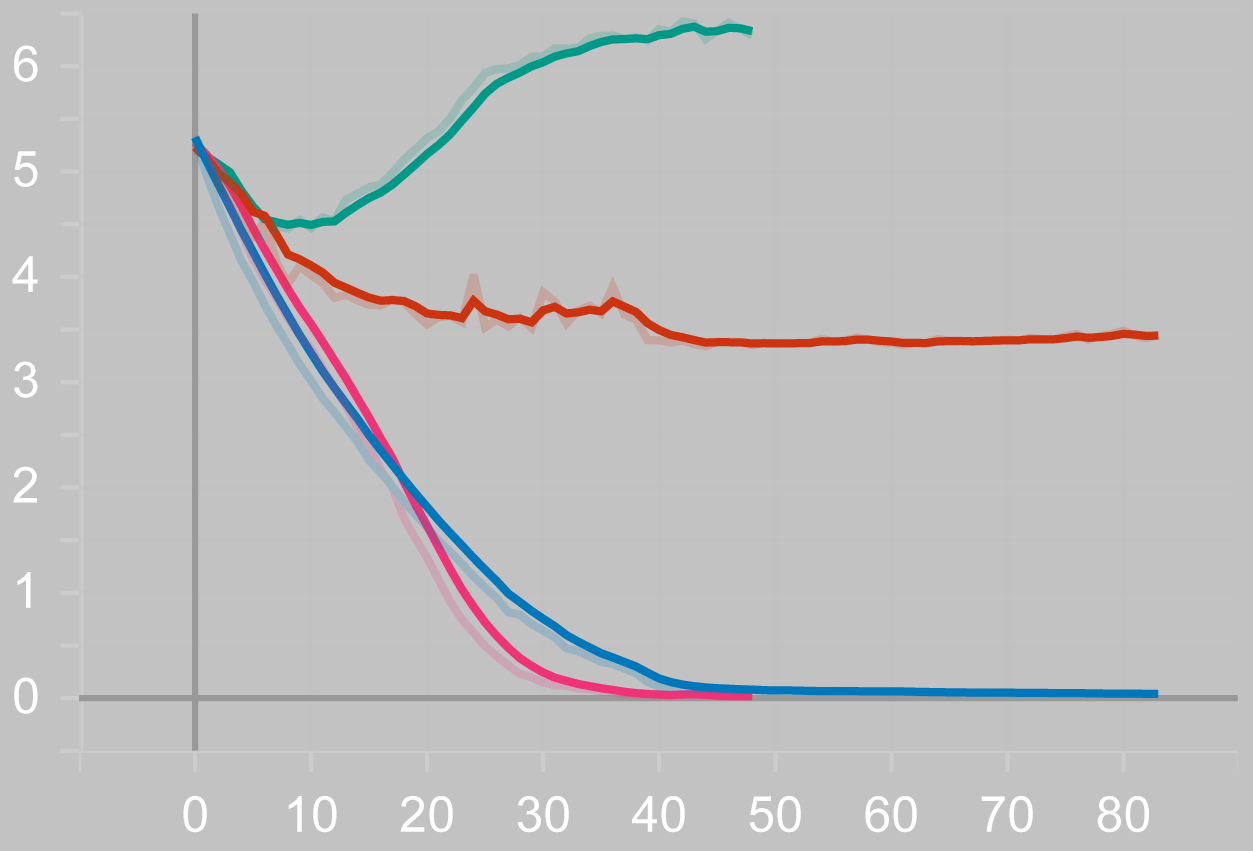
\includegraphics[width=240]{res/data_loss.png}
    \caption{Comparison of training and validation loss for ResNet and Vision Transformer (ViT) models.}
    \label{fig:loss_comparison}
\end{figure}

The results indicate that the Vision Transformer model converges faster and achieves lower validation loss compared to ResNet, demonstrating its superior performance in capturing global dependencies and generalizing to unseen data.

\subsection{Discussion}
The experimental results highlight several key insights:
\begin{itemize}
    \item The use of pretrained models significantly improves the initial performance and speeds up convergence.
    \item The Vision Transformer model outperforms ResNet in terms of both accuracy and loss, showcasing the effectiveness of self-attention mechanisms in handling complex datasets.
    \item Data augmentation through DCGAN provides a valuable boost in model performance by increasing the diversity of the training data.
\end{itemize}

\subsection{Ablation Studies}
To further understand the impact of different components of our methodology, we conducted ablation studies by systematically removing or altering specific elements and observing the effects on model performance. These studies confirmed the critical importance of pretrained models, data augmentation, and hyperparameter tuning in achieving optimal results.

%$\TODO{Include further experiments, such as the impact of different data augmentation strategies and detailed analysis of hyperparameter sensitivity.}
